\documentclass{article}

\UseRawInputEncoding

\usepackage[portuges]{babel}
\usepackage[utf8]{inputenc} 
\usepackage{fancyhdr}
\usepackage{graphicx} 
\usepackage{titling} 
\usepackage{indentfirst}
\usepackage{listings}
\usepackage{color}
\usepackage{xcolor}

\definecolor{codegreen}{rgb}{0,0.6,0}
\definecolor{codegray}{rgb}{0.5,0.5,0.5}
\definecolor{codepurple}{rgb}{0.58,0,0.82}
\definecolor{backcolour}{rgb}{0.95,0.95,0.92}

\lstdefinestyle{mystyle}{
  backgroundcolor=\color{backcolour},   commentstyle=\color{codegreen},
  keywordstyle=\color{magenta},
  numberstyle=\tiny\color{codegray},
  stringstyle=\color{codepurple},
  basicstyle=\ttfamily\footnotesize,
  breakatwhitespace=false,         
  breaklines=true,                 
  captionpos=b,                    
  keepspaces=true,                 
  numbers=left,                    
  numbersep=5pt,                  
  showspaces=false,                
  showstringspaces=false,
  showtabs=false,                  
  tabsize=2
}

\lstset{style=mystyle}

\parindent=0pt
\parskip=2pt

\newcommand{\subtitle}[1]{%
  \posttitle{%
    \par\end{center}
    \begin{center}\large#1\end{center}
    \vskip0.5em}%
}
\graphicspath{ {./images/} }

\rfoot{\thepage}

\pagenumbering{arabic}

%%%%%%%%%%%%%%%%%%%%%%%%%%%%%%%%%%%%%%%%%%%%%%%%%%%%%%%%%%%
\title{Trabalho Prático 2} %Titulo do documento

\subtitle{Processamento de Linguagens e Compiladores}

\author{Bárbara Faria\\A85774
        \and            
        José Pires\\A84552
        \and 
        Tiago Lima\\A85126} %autores do documento
\date{ (\today)} %data

\begin{document} % corpo do documento

\maketitle %apresentar titulo, autor e data

\begin{center}%Imagens 

\includegraphics[width=0.4\textwidth]{Uminho.jpg} 
\end{center}

\clearpage %Deixar a página branca até o próximo tema
%%%%%%%%%%%%%%%%%%%%%%%%%%%%%%%%%%%%%%%%%%%%%%%%%%%%%%%%%%%

\tableofcontents % Insere a tabela de indice
\clearpage %Deixar a página branca até o próximo tema

%%%%%%%%%%%%%%%%%%%%%%%%%%%%%%%%%%%%%%%%%%%%%%%%%%%%%%%%%%%

\section{Introdução} \label{sec:Introdução} %etiqueta para fazer referência cruzada às secçoes
\setlength{\parindent}{5ex} Este trabalho tem como objetivo desenvolver um compilador para a nossa própria linguagem, fazendo a tradução entre o código da nossa linguagem, de acordo com as regras estipuladas para a mesma, para código {\tt Assembly} da {\tt VM}.
\par Para atingir este objetivo, foi desenvolvido um analisador lexical com o Lex, que retorna uma lista de tokens para um analisador semântico, desenvolvido em yacc. Este analisador semântico por sua vez traduz a linguagem para o código executável final {\tt Assembly} da {\tt VM}.
\clearpage



%%%%%%%%%%%%%%%%%%%%%%%%%%%%%%%%%%%%%%%%%%%%%%%%%%%%%%%%%%%

\section{Sintaxe da Linguagem} \label{sec:Sintaxe da Linguagem}
\setlength{\parindent}{5ex} O desenvolvimento da nossa linguagem de programação imperativa teve inspiração em duas já conhecidas: C e Python.


%%%%%%%%%%%%%%%%%%%%%%%%%%%%%%%%%%%%%%%%%% 2.1


\subsection{Declaração de variáveis e atribuições}
\setlength{\parindent}{5ex} Variáveis do mesmo tipo podem ser declaradas numa única linha. Esta deve começar com o tipo correspondente seguido de uma seta (\textbf{-\textgreater}) para indicar o início da declaração e terminar com um ponto e vírgula acompanhado de uma mudança de linha. Um aspecto muito importante é que as declarações devem ser feitas antes de qualquer instrução. É também permitida a atribuição de um valor quando se declara uma variável do tipo inteiro. Caso contrário, é-lhe atribuída o valor 0.
\par A linguagem também suporta \textbf{arrays}. É necessário que lhes seja atribuído um valor para indicar as suas dimensões ou uma lista com os valores que os vão constituir. No primeiro caso o arrays são preenchidos com o valor 0.
\par Para realizar atribuições usa-se o símbolo \textbf{":"}.

\par Exemplo de declarações:
\begin{lstlisting}[firstnumber=0]
Int -> x:5, y;
Array -> a:10, b:[1,2,3,-4,-5];
\end{lstlisting}

\par Exemplo de atribuições:
\begin{lstlisting}[firstnumber=0]
x : 6;
y : -7;
a[2] : 5;
a[x] : 7;
y : b[0];
\end{lstlisting}

\par Neste programa, temos duas variáveis do tipo inteiro: \textbf{x} e \textbf{y}. A primeira tem o valor 5 e a segunda o valor 0.
Para além disso, foram criados dois \textbf{arrays}: \textbf{a} e \textbf{b}. O primeiro tem tamanho 10 e foi preenchido a zeros; o segundo tem tamanho 5 e contém os valores 1,2,3,-4 e -5.



%%%%%%%%%%%%%%%%%%%%%%%%%%%%%%%%%%%%%%%%%% 2.2

\subsection{Cálculo de Expressões}
\setlength{\parindent}{5ex} Para o cálculo de expressões, as seguintes operações são permitidas (por ordem crescente de prioridade):

\begin{description}
\item[1)] Operações booleanas: conjunção (\textbf{and}), disjunção (\textbf{or}) e negação (\textbf{!});
\item[2)] Operações de verificação de igualdade/desigualdade: igual (\textbf{=}), diferente (\textbf{!=}), maior ({\tt >}), menor ({\tt <}), maior ou igual ({\tt >=}) e menor ou igual ({\tt <=});
\item[3)] Operações sobre inteiros de soma (\textbf{+}) e subtracção (\textbf{-});
\item[4)] Operações sobre inteiros de multiplicação (\textbf{*}), divisão (\textbf{/}) e o resto da divisão inteira (\textbf{\%});
\item[5)] Uso de \textbf{'('} e \textbf{')'} para definir uma maior prioridade de operações.
\end{description}

Exemplo de uma atribuição a uma variável:
\begin{lstlisting}[firstnumber=0]
z : 4*(y-2) and (y!=0 or x>=4);
\end{lstlisting}
A variável z ficará com o valor lógico daquela expressão. 
\par Mais uma vez, as atribuições devem terminar com um ponto e vírgula seguidas de uma mudança de linha.

%%%%%%%%%%%%%%%%%%%%%%%%%%%%%%%%%%%%%%%%%%%%%%% 2.3

\subsection{Standard input e output}
\setlength{\parindent}{5ex} Para fazer a leitura e escrita devem ser utilizadas as funções \textbf{read} e \textbf{write}. 
\par A função \textbf{read} pode receber um ou nenhum argumento. No primeiro caso, é lhe passada uma string entre aspas, que será imprimida no ecrã. Esta função só pode ser utilizada numa atribuição, isto é, o utilizador escreve um valor e este será reclamado por uma variável. Por exemplo:
\begin{lstlisting}[firstnumber=0]
x:read();
y:read("Valor de y:");
\end{lstlisting}

\par A função \textbf{write} pode receber como argumento uma string entre aspas. Também pode receber uma string, seguida de variáveis (estando estes argumentos separados por virgula). Ou ainda, aceita apenas uma variável como argumento. Tal como o nome indica, o propósito desta função é imprimir no ecrã as strings e o valor das variáveis (no caso dos arrays, imprime o array completo).

\begin{lstlisting}[firstnumber=0]
write(x);
write("Valores de x e y:",x,y);
write("Adoro PLC");
\end{lstlisting}

%%%%%%%%%%%%%%%%%%%%%%%%%%%%%%%%%%%%%%%%%%%%%%% 2.4

\subsection{Condicionais}
\setlength{\parindent}{5ex} A definição de condicionais é feita através dos símbolos \textbf{?} e \textbf{-\textgreater\textgreater}. O primeiro símbolo equivale ao \textbf{if} e o segundo ao \textbf{else}. Há duas maneiras de usar os condicionais:

\begin{description}
\item[1)] Apenas com o \textbf{?} (caso \textbf{if then}): o símbolo é seguido de uma expressão dentro de parêntesis curvos (condição) que por sua vez é sucedida por uma seta e uma mudança de linha. Depois escrevem-se as instruções e fecha-se com um ponto e virgula. Todas as instruções devem terminar por um ponto e virgula e uma mudança de linha.
\item[2)] Usando os dois símbolos (caso \textbf{if then else}): aplicam-se as regras anteriores, no entanto quando se fecha o \textbf{if} com o ponto virgula, acrescenta-se o símbolo \textbf{-\textgreater\textgreater} acompanhado de uma mudança de linha. Escrevem-se as instruções respeitando as normas mencionadas acima. Para terminar, escreve-se um ponto e virgula para indicar o fim do \textbf{else}.
\end{description}

Exemplo de condicionais:
\begin{lstlisting}[firstnumber=0]
?(x<=3 and y>5)->
    x:x+y;
;

?(x=6 or y!=7)->
    x:x*(y+1);
    y:read("Novo valor de y:");
;->>
    x:x*(y-1);
;
\end{lstlisting}

%%%%%%%%%%%%%%%%%%%%%%%%%%%%%%%%%%%%%%%%%%%%%%% 2.5

\subsection{Ciclos}
\setlength{\parindent}{5ex} Para os ciclos, foi implementado o \textbf{while-do}. A sua definição é feita através do símbolo \textbf{W?} seguido de uma expressão entre parêntesis curvos (condição). Esta é sucedida por uma seta e uma mudança linha. Dá-se, então, inicio ao corpo do ciclo, o qual deve terminar por um ponto e virgula e uma mudança de linha. Este é constituído por instruções que devem respeitar as regras estabelecidas nos condicionais.

Exemplo de ciclos:
\begin{lstlisting}[firstnumber=0]
W?(x<=5)->
    write(x);
    x:x+1;
;
\end{lstlisting}

%%%%%%%%%%%%%%%%%%%%%%%%%%%%%%%%%%%%%%%%%%%%%%% 2.6

\subsection{Main}
\setlength{\parindent}{5ex} Depois de declarar variáveis, é necessário usar a palavra reservada \textbf{Main} seguida de uma seta para indicar o início das instruções. As intruções mais uma vez devem terminar por ponto e virgula seguido de uma mudança de linha. Para fechar o \textbf{Main} usa-se um ponto e virgula.

Exemplo de um programa:
\begin{lstlisting}[firstnumber=0]
Int -> x:5;

Main ->
    W?(x<=5)->
        write(x);
        x:x+1;
    ;
;
\end{lstlisting}
(Nota: a indentação é puramente estética)
\vspace{1CM}

%%%%%%%%%%%%%%%%%%%%%%%%%%%%%%%%%%%%%%%%%%%%%%%%%%%%%%%%%%% 3
\section{Concepção/Resolução} \label{sec:Concepção/Resolução}

%%%%%%%%%%%%%%%%%%%%%%%%%%%%%%%%%%%%%%%%%%%% 3.1

\subsection{Analisador Léxico - Lex}
\setlength{\parindent}{5ex}Inicialmente foi criado um analisador léxico, utilizando a ferramenta \textbf{lex}, que permite processar o código fonte. Durante este processamento, são retornados diferentes \textbf{tokens}, que correspondem a expressões regulares com o propósito de identificar padrões no código.
\par Em programação de computadores, uma palavra reservada é uma palavra que não pode ser utilizada como um identificador por ser reservada para uso da gramática da linguagem. Assim quando estas são identificadas, os seus \textbf{tokens} são devolvidos.
\par Palavras reservadas:

\begin{lstlisting}[]
def t_MAIN(t):
    r'Main'
    return t

def t_INT(t):
    r'Int'
    return t

def t_ARR(t):
    r'Array'
    return t

def t_WRITE(t):
    r'write'
    return t

def t_READ(t):
    r'read'
    return t
    
def t_AND(t):
    r'and'
    return t

def t_OR(t):
    r'or'
    return t
\end{lstlisting}

Para possibilitar a declaração de variáveis e números inteiros, utilizam-se as seguintes expressões regulares:
\begin{lstlisting}[]
t_ID = r'[a-z][a-zA-Z]*'

def t_NUMI(t):
    r'[0-9]+'
    t.value = int(t.value)
    return t
\end{lstlisting}
Os nomes das variáveis são obrigados a começar por letra minúscula podem ser sucedidos por uma ou mais letras.

\par Os \textbf{tokens} que identificam os condicionais e os ciclos são os seguintes:
\begin{lstlisting}[]
t_IF = r'\?'

def t_ELSE(t):
    r'\->>'
    return t
    
def t_WHILE(t):
    r'W\?'
    return t
\end{lstlisting}

De forma a identificar operados lógicos e aritméticos, usamos as seguintes expressões:
\begin{lstlisting}[]
t_EQ = r'\='
t_MAIOR = r'\>'
t_MENOR = r'\<'
t_MENOS = r'\-'
t_MAIS = r'\+'
t_MUL = r'\*'
t_DIV = r'\/'
t_RESDI = r'\%'

def t_NEQ(t):
    r'\!\='
    return t
    
def t_LE(t):
    r'\<\='
    return t

def t_GE(t):
    r'\>\='
    return t
\end{lstlisting}

Se for detetada um string é devolvido o seguinte \textbf{token}:
\begin{lstlisting}[]
def t_STRING(t):
    r'\"[^\"]*\"'
    return t
\end{lstlisting}

A negação de um valor é identificada pela seguinte expressão:
\begin{lstlisting}[]
def t_NOT(t):
    r'\!'
    return t
\end{lstlisting}

Os tokens abaixo detetam símbolos como o ponto e virgula, dois pontos...:
\begin{lstlisting}[]
t_PV = r';'
t_VIR = r','
t_DP = r':'
t_LPAREN = r'\('
t_RPAREN = r'\)'
t_LPARENR = r'\['
t_RPARENR = r'\]'
t_SETA = r'\->'
\end{lstlisting}

Para detectar novas linhas, a seguinte expressão é usada:
\begin{lstlisting}[]
def t_NL(t):
    r'\n'
    t.lexer.lineno += len(t.value)
    return t
\end{lstlisting}

Espaços e {\tt tabs} são ignorados:
\begin{lstlisting}[]
t_ignore = ' \t'
\end{lstlisting}

\vspace{1CM}

%%%%%%%%%%%%%%%%%%%%%%%%%%%%%%%%%%%%%%%%%%%%%% 3.2

\subsection{Estruturas de Dados / Variáveis Globais}
\setlength{\parindent}{5ex} O grupo optou por criar um dicionário chamado \textbf{tabID} onde iremos guardar informação sobre as variáveis declaradas no programa, com o intuito de verificar e avisar o utilizador de possíveis erros no seu código, assim como realizar operações sobre essas variáveis.
\par A informação que queremos armazenar é a seguinte:
\begin{description}
\item[1)] O \textbf{nome} de uma variável;

\item[2)] O \textbf{tipo} de uma variável (\textbf{Int} ou \textbf{Array});

\item[3)] O endereço (\textbf{stack pointer}) de uma variável;

\item[4)] O \textbf{tamanho} ou \textbf{valor} de uma variável, caso o tipo desta seja \textbf{Array} ou \textbf{Int}, respectivamente.
\end{description}

Os elementos do dicionário serão constituídos por conjuntos chave-valor. Neste caso a chave será o \textbf{nome} de uma variável e os valor será um tuplo da forma: \textbf{(endereço, valor/tamanho, tipo)}

\par Também recorremos à ajuda de três variáveis: \textbf{proxE}, \textbf{nivelC} e \textbf{conta}.

\begin{lstlisting}[]
parser.tabID = {}   
parser.proxE = 0
parser.nivelC = 0
parser.conta = 0
\end{lstlisting}

%%%%%%%%%%%%%%%%%%%%%%%%%%%%%%%%%%%%%%%%%%%%%%%%% 3.3

\subsection{Analisador Semântico - Yacc}
\setlength{\parindent}{5ex}Depois de detetar os \textbf{tokens} é necessário estabelecer regras relativamente à sua organização: sintaxe da linguagem.

%%%%%%%%%%%%%%%%%%%%%%%%%%%%%%%%%%%%%%%%%%%%%%%% 3.3.1

\subsubsection {Declaração de variáveis}
\setlength{\parindent}{5ex}Um programa pode ter zero ou mais declarações. As seguintes produções traduzem isso:
\begin{lstlisting}[firstnumber=13]
def p_decls(p):
    "Decls : Decls Decl"
    p[0] = p[1] + p[2]

def p_decls_empty(p):
    "Decls : "
    p[0] = ''
\end{lstlisting}

\par Podemos ter dois tipos de declarações: Inteiros ou Arrays. Tal como foi especificado na secção 2.1, uma declaração tem de começar pelo respectivo tipo seguido de uma seta e terminar num ponto e virgula. Declarações do mesmo tipo podem ser feitas numa única linha.

\begin{lstlisting}[firstnumber=22]
def p_decl_int(p):
    "Decl : INT SETA DeclList PV NL"
    p[0] = p[3]

def p_decl_array(p):
    "Decl : ARR SETA ArrayList PV NL"
    p[0] = p[3]

def p_decl_nl(p):
    "Decl : NL"
    p[0] = ''


def p_decllist(p):
    "DeclList : UniDecl VIR DeclList"
    p[0] = p[1] + p[3]

def p_decllist_uni(p):
    "DeclList : UniDecl"
    p[0] = p[1]

def p_arraylist(p):
    "ArrayList : Array VIR ArrayList"
    p[0] = p[1] + p[3]

def p_arraylist_uni(p):
    "ArrayList : Array"
    p[0] = p[1]
\end{lstlisting}

\par Uma variável inteira pode ser declarada de 2 formas diferentes: não lhe atribuindo um valor (neste caso irá ser 0) ou atribuindo-lhe um número inteiro. No momento da declaração é inserida no dicionário \textbf{tabID} a sua informação, após a verificação de possíveis conflitos de re-declarações. Neste ponto recorremos ao auxilio da variável global \textbf{proxE} para determinar o endereço da variável.
\par No caso em que não há atribuição de valor, é efetuado um \textbf{PUSHI 0} que empilha na Stack o valor 0. Caso haja atribuição, é realizado um \textbf{PUSHI str(p[3])}, onde p[3] corresponde ao simbolo terminal \textbf{NUMI} (se for um número negativo será \textbf{PUSHI str(-p[4])}) que empilhará o valor correspondente na pilha.

\clearpage
\begin{lstlisting}[firstnumber=52]
def p_unidecl_id(p): 
    "UniDecl : ID"
    if p[1] in parser.tabID:
        string = "Erro semântico: Var " + p[1] + " já está definida!"
        p[0] = r'ERR "' + string + '"' + '\n' + 'STOP' + '\n'
    
    else:
        parser.tabID.update({p[1] : (parser.proxE,0,"Int")})
        parser.proxE += 1
        p[0] = r'PUSHI 0' + '\n'


def p_unidecl_atr(p):
    "UniDecl : ID DP NUMI"
    if p[1] in parser.tabID:
        string = "Erro semântico: Var " + p[1] + " já está definida!"
        p[0] = r'ERR "' + string + '"' + '\n' + 'STOP' + '\n'
    
    else:
        parser.tabID.update({p[1] : (parser.proxE,p[3],"Int")})
        parser.proxE += 1
        p[0] = r'PUSHI '+ str(p[3]) + '\n'


def p_unidecl_atrn(p):
    "UniDecl : ID DP MENOS NUMI"
    if p[1] in parser.tabID:
        string = "Erro semântico: Var " + p[1] + " já está definida!"
        p[0] = r'ERR "' + string + '"' + '\n' + 'STOP' + '\n'
    
    else:
        parser.tabID.update({p[1] : (parser.proxE,-p[4],"Int")})
        parser.proxE += 1
        p[0] = r'PUSHI '+ str(-p[4]) + '\n'
\end{lstlisting}

\par Um array pode ser declarado de 2 formas diferentes: atribuindo-lhe um valor N que será o seu tamanho (neste caso irá ser preenchido a 0) ou atribuindo-lhe uma lista de números inteiros. No momento da declaração é inserida no dicionário \textbf{tabID} a sua informação, após a verificação de possíveis conflitos de re-declarações. Neste ponto recorremos ao auxilio da variável global \textbf{proxE} para determinar o endereço da variável.
\par No caso em que há atribuição de tamanho, é efetuado um \textbf{PUSHN str(p[3])} que empilha na Stack o valor 0 N vezes (sendo N o tamanho do array). Caso haja atribuição de uma lista, iremos percorrer a mesma e, em cada valor, realizar um \textbf{PUSHI str(p[1])}, onde p[1] corresponde ao simbolo terminal \textbf{NUMI} (se for um número negativo será \textbf{PUSHI str(-p[2])}) que empilhará o valor correspondente na pilha. 
\par Durante a travessia da lista, recorremos à variável global \textbf{conta} para nos ajudar a determinar o endereço do array.

\clearpage
\begin{lstlisting}[firstnumber=88]
def p_arrayAtr(p):
    "Array : ID DP NUMI"
    if p[1] in parser.tabID:
        string = "Erro semântico: Var " + p[1] + " já está definida!"
        p[0] = r'ERR "' + string + '"' + '\n' + 'STOP' + '\n'
    
    else:
        parser.tabID.update({p[1] : (parser.proxE,p[3],"Array")})    #(end do inicio do array,tamanho,tipo da var Array)
        parser.proxE += p[3]
        p[0] = r'PUSHN ' + str(p[3]) + '\n'


def p_arrayAtrlist(p):
    "Array : ID DP List"
    if p[1] in parser.tabID:
        string = "Erro semântico: Var " + p[1] + " já está definida!"
        p[0] = r'ERR "' + string + '"' + '\n' + 'STOP' + '\n'
    
    else:
        p[0] = p[3]
        parser.tabID.update({p[1] : (parser.proxE-parser.conta,parser.conta,"Array")})
        parser.conta = 0

def p_arrayAtrlist2(p):
    "List : LPARENR Nums RPARENR"
    p[0] = p[2]

def p_elems(p):
    "Nums : Nums VIR Num"
    parser.conta += 1
    p[0] = p[1] + p[3]

def p_elems2(p):
    "Nums : Num"
    parser.conta = 1
    p[0] = p[1]

def p_elems3(p):
    "Num : NUMI"
    p[0] = r'PUSHI ' + str(p[1]) + '\n'
    parser.proxE += 1

def p_elems4(p):
    "Num : MENOS NUMI"
    p[0] = r'PUSHI ' + str(-p[2]) + '\n'
    parser.proxE += 1
\end{lstlisting}
\clearpage

%%%%%%%%%%%%%%%%%%%%%%%%%%%%%%%%%%%%%%%%%%%%%%% 3.3.2

\subsubsection {Main}
\setlength{\parindent}{5ex}
Depois de declarar variáveis iniciam-se as instruções do programa. Estas encontram-se dentro da função Main. Assim, nesta secção iremos afetar o valor do registo \textbf{sp} (stack pointer) ao registo \textbf{fp} (frame pointer) através da instrução \textbf{START}. 
\par Um programa pode ter 0 ou mais instruções. Estas podem ser \textbf{Atribuições}, \textbf{Condições}, \textbf{Ciclos}, chamadas da função \textbf{write}. Cada instrução deve terminar por ponto e virgula seguido de uma mudança de linha. No fim, o programa pára, recorrendo à instrução \textbf{STOP}.

\begin{lstlisting}[firstnumber=137]
def p_main(p):
    "Main : MAIN SETA NL Instrs PV"
    p[0] = r'START' + '\n' + p[4] + r'STOP'



def p_instrs(p):
    "Instrs : Instrs Instr"
    p[0] = p[1] + p[2]

def p_instrs_empty(p):
    "Instrs : "
    p[0] = ''


def p_instr_atr(p):
    "Instr : Atr NL"
    p[0] = p[1]

def p_instr_cond(p):
    "Instr : Cond NL"
    p[0] = p[1]

def p_instr_ciclo(p):
    "Instr : Ciclo NL"
    p[0] = p[1]

def p_instr_write(p):
    "Instr : Write NL"
    p[0] = p[1]

def p_instr_nl(p):
    "Instr : NL"
    p[0] = ''
\end{lstlisting}

%%%%%%%%%%%%%%%%%%%%%%%%%%%%%%%%%%%% 3.3.3

\subsubsection {Atribuições}
\setlength{\parindent}{5ex} A nossa linguagem permite fazer atribuições a variáveis inteiras ou a posições de arrays. O compilador irá verificar possíveis erros tais como chamar variáveis que não existem, ou acessos a uma posição que não pertence ao array.
\par A seguinte produção permite atribuir o valor de uma expressão a uma variável inteira:

\begin{lstlisting}[firstnumber=174]
def p_atrib(p):
    "Atr : ID DP Expr PV"
    if p[1] not in parser.tabID:
        string = "Erro semântico: Var " + str(p[1]) + " não está definida!"
        p[0] = r'ERR "' + string + '"' + '\n' + 'STOP' + '\n'

    elif parser.tabID[p[1]][2]!="Int":
        string = "Erro semântico: Var " + str(p[1]) + " não é do tipo inteiro!"
        p[0] = r'ERR "' + string + '"' + '\n' + 'STOP' + '\n'     
    
    else:
        p[0] = p[3] + r'STOREG ' + str(parser.tabID[p[1]][0]) + '\n'
\end{lstlisting}

Recorrendo à instrução \textbf{STOREG} guardamos o valor da expressão (p[3]) no endereço da variável, que pode ser encontrado no dicionário \textbf{tabID} na posição 0 do tuplo associado ao nome da variável.

\par A produção seguinte permite fazer atribuições a variáveis inteiras usando a função \textbf{read}:

\begin{lstlisting}[firstnumber=188]
ef p_atrib_read(p):
    "Atr : ID DP Read"
    if p[1] not in parser.tabID:
        string = "Erro semântico: Var " + str(p[1]) + " não está definida!"
        p[0] = r'ERR "' + string + '"' + '\n' + 'STOP' + '\n'

    elif parser.tabID[p[1]][2]!="Int":
        string = "Erro semântico: Var " + str(p[1]) + " não é do tipo inteiro!"
        p[0] = r'ERR "' + string + '"' + '\n' + 'STOP' + '\n'

    else:
        p[0] = p[3] + r'STOREG ' + str(parser.tabID[p[1]][0]) + '\n'
\end{lstlisting}

Utilizando a instrução \textbf{STOREG} guardamos o valor do standard input (p[3]) no endereço da variável, que pode ser encontrado no dicionário \textbf{tabID} na posição 0 do tuplo associado ao nome da variável.

Além de variáveis inteiras, a nossa linguagem também permite fazer atribuições a posições de arrays (semelhante ao C, usa-se um número inteiro entre parênteses rectos depois do nome do array, para aceder a uma dada posição). A produção abaixo possibilita a atribuição a posições especificas de um array, isto é, \textbf{array[2] : Expr} :

\begin{lstlisting}[firstnumber=202]
def p_atribarray_numi(p):
    "Atr : ID LPARENR NUMI RPARENR DP Expr PV"
    if p[1] not in parser.tabID:
        string = "Erro semântico: Var " + str(p[1]) + " não está definida!"
        p[0] = r'ERR "' + string + '"' + '\n' + 'STOP' + '\n'

    elif parser.tabID[p[1]][2]!="Arr":
        string = "Erro semântico: Var " + str(p[1]) + " não é do tipo array!"
        p[0] = r'ERR "' + string + '"' + '\n' + 'STOP' + '\n'

    elif p[3]>=parser.tabID[p[1]][1]:
        string = "Erro semântico: " + p[3] + " encontra-se fora do limite do tamanho do array!"
        p[0] = r'ERR "' + string + '"' + '\n' + 'STOP' + '\n'

    else:
        p[0] = p[6] + r'STOREG ' + str(parser.tabID[p[1]][0]+p[3]) + '\n'
\end{lstlisting}

Mais um vez, a intrução \textbf{STOREG} é usada juntamente com o endereço do array mais o número que se encontra entre parênteses rectos.

\par Também é possível realizar o passo anterior mas em vez de atribuirmos o valor de uma expressão, o programa lê um valor do standard input. O armazenamento faz-se de maneira igual à anterior.

\begin{lstlisting}[firstnumber=220]
"Atr : ID LPARENR NUMI RPARENR DP Read"
    if p[1] not in parser.tabID:
        string = "Erro semântico: Var " + str(p[1]) + " não está definida!"
        p[0] = r'ERR "' + string + '"' + '\n' + 'STOP' + '\n'

    elif parser.tabID[p[1]][2]!="Array":
        string = "Erro semântico: Var " + str(p[1]) + " não é do tipo array!"
        p[0] = r'ERR "' + string + '"' + '\n' + 'STOP' + '\n'

    else:
        p[0] = p[6] + r'STOREG ' + str(parser.tabID[p[1]][0]+p[3]) + '\n'
\end{lstlisting}

Para atribuir um valor (seja este uma expressão ou vindo do standard input) a uma posição do array usando uma variável como indice, o processo complica um pouco. Primeiro temos de usar a instrução \textbf{PUSHGP} para empilhar o valor do regist \textbf{gp} (global pointer). De seguida empilhamos o valor do endereço do array (que se encontra na posição 0 do tuplo associado ao nome deste), através do comando \textbf{PUSHI}. Logo após, recorremos à instrução \textbf{PADD} que vai somar o endereço de gp com o inteiro correspondente ao endereço do array e empilhar esse resultado. Efetivamente temos na pilha o endereço do array. A seguir aplicamos a instrução \textbf{PUSHG} para empilhar o valor da variável que irá ser usada como índice. Com o \textbf{CHECK} verificamos se o valor no topo da pilha está dentro do intervalo [0 - (Tamanho do array -1)], o que nos permite lançar a mensagem de erro "Index out of order". O proximo passo é empilhar o resultado da expressão ou o valor que o programa leu do standard input e aplicar a instrução \textbf{STOREN}.
As seguintes produções retratam este processo:

\begin{lstlisting}[firstnumber=234]
def p_atribarray_id(p):
    "Atr : ID LPARENR ID RPARENR DP Expr PV"
    if p[1] not in parser.tabID:
        string = "Erro semântico: Var " + str(p[1]) + " não está definida!"
        p[0] = r'ERR "' + string + '"' + '\n' + 'STOP' + '\n'

    elif parser.tabID[p[1]][2]!="Array":
        string = "Erro semântico: Var " + str(p[1]) + " não é do tipo array!"
        p[0] = r'ERR "' + string + '"' + '\n' + 'STOP' + '\n'

    elif p[3] not in parser.tabID:
        string = "Erro semântico: Var " + str(p[3]) + " não está definida!"
        p[0] = r'ERR "' + string + '"' + '\n' + 'STOP' + '\n'

    elif parser.tabID[p[3]][2]!="Int":
        string = "Erro semântico: Var " + str(p[1]) + " não é do tipo inteiro!"
        p[0] = r'ERR "' + string + '"' + '\n' + 'STOP' + '\n'

    else:
        p[0] = r'PUSHGP' + '\n' + \
               r'PUSHI ' + str(parser.tabID[p[1]][0]) + '\n' + \
               r'PADD' + '\n' + \
               r'PUSHG ' + str(parser.tabID[p[3]][0]) + '\n' + \
               r'CHECK ' + '0 ' + str(parser.tabID[p[1]][1]-1) + '\n' + \
               p[6] + \
               r'STOREN' + '\n'


def p_atribarray_read(p):
    "Atr : ID LPARENR ID RPARENR DP Read"
    if p[1] not in parser.tabID:
        string = "Erro semântico: Var " + str(p[1]) + " não está definida!"
        p[0] = r'ERR "' + string + '"' + '\n' + 'STOP' + '\n'

    elif parser.tabID[p[1]][2]!="Array":
        string = "Erro semântico: Var " + str(p[1]) + " não é do tipo array!"
        p[0] = r'ERR "' + string + '"' + '\n' + 'STOP' + '\n'

    elif p[3] not in parser.tabID:
        string = "Erro semântico: Var " + str(p[3]) + " não está definida!"
        p[0] = r'ERR "' + string + '"' + '\n' + 'STOP' + '\n'

    elif parser.tabID[p[3]][2]!="Int":
        string = "Erro semântico: Var " + str(p[1]) + " não é do tipo inteiro!"
        p[0] = r'ERR "' + string + '"' + '\n' + 'STOP' + '\n'

    else:
        p[0] = r'PUSHGP' + '\n' + \
               r'PUSHI ' + str(parser.tabID[p[1]][0]) + '\n' + \
               r'PADD' + '\n' + \
               r'PUSHG ' + str(parser.tabID[p[3]][0]) + '\n' + \
               r'CHECK ' + '0 ' + str(parser.tabID[p[1]][1]) + '\n' + \
               p[6] + \
               r'STOREN' + '\n'
\end{lstlisting}

%%%%%%%%%%%%%%%%%%%%%%%%%%%%%%%%%%%%%%%%%%%%%%% 3.3.4

\subsubsection {Read}
\setlength{\parindent}{5ex}
A função \textbf{read} pode receber uma string ou nada como argumento. Em ambos os casos o utilizador deve dar uso aos parênteses curvos depois da sua chamada, i.e., \textbf{read(args)}. Caso não hajam argumentos, será apenas necessário usar o comando \textbf{READ} da VM, seguido da instrução \textbf{ATOI} para converter o valor lido para um inteiro. Se o utilizador passar uma string como argumento, é necessário utilizar os comandos \textbf{PUSHS}, para empilhar a string na heap, e \textbf{WRITES} que irá imprimi-la no standard output. Seguidamente, aplica-se o mesmo processo descrito no caso acima.
\par As seguintes produções descrevem este processo:

\begin{lstlisting}[firstnumber=291]
def p_read(p):
    "Read : READ LPAREN RPAREN PV"
    p[0] = r'READ' + '\n' + r'ATOI' + '\n'

def p_read_String(p):
    "Read : READ LPAREN String RPAREN PV"
    p[0] = r'PUSHS ' + p[3] + '\n' + r'WRITES' + '\n' + \
           r'PUSHS ' + r'"\n"' + '\n' + r'WRITES' + '\n' + \
           r'READ' + '\n' + r'ATOI' + '\n'
\end{lstlisting}
O símbolo não terminal \textbf{String} abrange as strings definidas no \textbf{token STRING}:

\begin{lstlisting}[firstnumber=356]
def p_string(p):
    "String : STRING"
    p[0] = str(p[1])
\end{lstlisting}

%%%%%%%%%%%%%%%%%%%%%%%%%%%%%%%%%%%%%%%%%%%%%%% 3.3.5

\subsubsection {Write}
\setlength{\parindent}{5ex} Tal como na função \textbf{read}, será obrigatório fazer uso dos parêntesis curvos para indicar os argumentos a ser servidos. Estes podem ser simplesmente uma \textbf{string}, para a qual usaremos os comandos \textbf{PUSHS} seguido de \textbf{WRITES} para traduzir em código da VM.
\par Também é permitido passar uma string como argumento seguida de variáveis do tipo inteiro, todas estas separadas por vírgulas. O símbolo não terminal \textbf{ListArgs} irá abranger as variáveis. Usando o mesmo processo descrito acima fazemos a tradução de escrever a string no standard output para código VM. Para as variáveis, recorremos aos comandos \textbf{PUSHG} e \textbf{WRITEI}.
\par Por ultimo é possível passar apenas uma variável como argumento e imprimir o valor desta (se for um array, imprime-o todo). Usufruindo das instruções \textbf{PUSHG} e \textbf{WRITEI}, fazemos a tradução para o código da VM.
\par As seguintes produções retratam o que foi descrito:

\begin{lstlisting}[firstnumber=330]
def p_write_string(p):
    "Write : WRITE LPAREN String RPAREN PV"   
    p[0] = r'PUSHS ' + p[3] + '\n' + r'WRITES' + '\n' + r'PUSHS ' + r'"\n"' + '\n' + r'WRITES' + '\n'

def p_write_args(p):
    "Write : WRITE LPAREN String VIR ListArgs RPAREN PV"
    p[0] = r'PUSHS ' + p[3] + '\n' + r'WRITES' + '\n' + r'PUSHS ' + r'"\n"' + '\n' + r'WRITES' + '\n' + p[5]

def p_write_id(p):
    "Write : WRITE LPAREN ID RPAREN PV"
    if p[3] not in parser.tabID:
        string = "Erro semântico: Var " + p[3] + " não está definida!" + '\n'
        p[0] = r'ERR "' + string + '"' + '\n' + 'STOP' + '\n'

    elif parser.tabID[p[3]][2]=="Int":
        p[0] = r'PUSHG ' + str(parser.tabID[p[3]][0]) + '\n' + r'WRITEI' + '\n' + r'PUSHS ' + r'"\n"' + '\n' + r'WRITES' + '\n'

    elif parser.tabID[p[3]][2]=="Array":
        aux = 0
        s = ''
        while aux<parser.tabID[p[3]][1]:
            s += r'PUSHG ' + str(parser.tabID[p[3]][0]+aux) + '\n' + r'WRITEI' + '\n' + r'PUSHS ' + r'"\n"' + '\n' + r'WRITES' + '\n'
            aux += 1
        p[0] = s


def p_string(p):
    "String : STRING"
    p[0] = str(p[1])

def p_listargs(p):
    "ListArgs : ListArgs VIR Elem"
    p[0] = p[1] + p[3]

def p_listargs_uno(p):
    "ListArgs : Elem"
    p[0] = p[1]


def p_elem_id(p):
    "Elem : ID"
    if p[1] not in parser.tabID:
        string = "Erro semântico: Var " + str(p[1]) + " não está definida!"
        p[0] = r'ERR "' + string + '"' + '\n' + 'STOP' + '\n'

    elif parser.tabID[p[1]][2]!="Int":
        string = "Erro semântico: Var " + str(p[1]) + " não é do tipo inteiro!"
        p[0] = r'ERR "' + string + '"' + '\n' + 'STOP' + '\n'

    else:
        p[0] = r'PUSHG ' + str(parser.tabID[p[1]][0]) + '\n' + r'WRITEI' + '\n' + r'PUSHS ' + r'"\n"' + '\n' + r'WRITES' + '\n'
\end{lstlisting}

%%%%%%%%%%%%%%%%%%%%%%%%%%%%%%%%%%%%%%%%%%%%% 3.3.6

\subsubsection {Condições}
\setlength{\parindent}{5ex} O \tetxbf{if} começa pelo  \textbf{token IF} seguido de uma expressão cujo valor lógico deve ser avaliado e de instruções no seu corpo. O \textbf{else} inicia com o \textbf{token ELSE} sucedido de instruções. Poderemos ter dois casos:

\begin{description}
\item[1)] Se o utilizador apenas usar o statement \textbf{if then} coloca-se uma label com o nome "E+nivelC" no topo da pilha. De seguida empilha-se o valor da expressão calculada seguido do comando \textbf{jz} com label "E+(nivelC+1)". Por fim o código das instruções do corpo do ciclo é empilhado mais a label "E+(nivelC+1)". Caso o valor da expressão seja falso, então a instrução \textbf{jz} faz o código saltar para o fim do ciclo. Caso contrário, o corpo deste é executado. Por fim incrementa-se o contador de labels \textbf{nivelC} em duas unidades.

\item[2)] Se o utilizador apenas usar o statement \textbf{if then else} coloca-se uma label com o nome "E+nivelC" no topo da pilha. 
De seguida empilha-se o valor da expressão calculada seguido do comando \textbf{jz} com a label "E+(nivelC+1)". Depois o código das instruções do \textbf{if} é empilhado acompanhado da instrução \textbf{JUMP} com label "E+(nivelC+2)". O próximo passo será colocar no topo da pilha a label "E+(nivelC+1)" sucedida do código das intruções do \textbf{else}. Por fim acrescenta-se a label "E+(nivelC+2)" e incrementa-se o contador de labels \textbf{nivelC} em três unidades. Caso a condição do \textbf{if} seja falsa é executado um \textbf{JUMP} para a label "E+(nivelC+1)", senão as instruções deste serão realizadas acompanhadas e ignora-se o \textbf{else}, fazendo um \textbf{JUMP} para a label "E+(nivelC+2)".

\end{description}
As produções abaixo descrevem este processo:

\begin{lstlisting}[firstnumber=303]
def p_cond_if(p):
    "Cond : IF LPAREN Expr RPAREN SETA NL Instrs PV"
    p[0] = r'E' + str(parser.nivelC) + r': nop' + '\n' + p[3] + \
           r'JZ E' + str(parser.nivelC + 1) + '\n' + p[7] + \
           r'E' + str(parser.nivelC + 1) + r': nop' + '\n'
    parser.nivelC += 2


def p_cond_ifelse(p):
    "Cond : IF LPAREN Expr RPAREN SETA NL Instrs PV ELSE NL Instrs PV"
    p[0] = r'E' + str(parser.nivelC) + r': nop' + '\n' + p[3] + \
           r'JZ E' + str(parser.nivelC + 1) + '\n' + p[7] + 'JUMP E' + str(parser.nivelC + 2) + '\n' + \
           r'E' + str(parser.nivelC + 1) + r': nop' + '\n' + p[11] + \
           r'E' + str(parser.nivelC + 2) + r': nop' + '\n'
    parser.nivelC += 3
\end{lstlisting}

%%%%%%%%%%%%%%%%%%%%%%%%%%%%%%%%%%%%%%%%%%%%%% 3.3.7

\subsubsection {Ciclos}
\setlength{\parindent}{5ex}Os ciclos começam pelo  \textbf{token WHILE} seguido de uma expressão cujo valor lógico deve ser avaliado e de instruções no seu corpo. Assim, a sua tradução para código da VM é muito semelhante ao caso \textbf{if then}. A única diferença é que no final de executarmos as instruções do corpo do ciclo é necessário realizar um \textbf{JUMP} para a label onde este foi iniciado. Abaixo podemos observar a produção correspondente:

\begin{lstlisting}[firstnumber=321]
def p_ciclo(p):
    "Ciclo : WHILE LPAREN Expr RPAREN SETA NL Instrs PV"
    p[0] = r'E' + str(parser.nivelC) + r': nop' + '\n' + p[3] + \
           r'JZ E' + str(parser.nivelC + 1) + '\n' + p[7] + 'JUMP E' + str(parser.nivelC) + '\n' + \
           r'E' + str(parser.nivelC + 1) + r': nop' + '\n'
    parser.nivelC += 2
\end{lstlisting}

%%%%%%%%%%%%%%%%%%%%%%%%%%%%%%%%%%%%%%%% 3.3.8

\subsubsection {Cálculo de expressões}
\setlength{\parindent}{5ex} Para implementar o cálculo de expressões definiram-se várias produções. Iremos explica-las por ordem crescente de prioridade. 
\par O grupo usou os símbolos não terminais \textbf{Expr} e \textbf{LExpr} juntamente com os \textbf{tokens AND, OR} e \textbf{NOT} para definir as operações booleanas. Visto não haver instruções \textbf{AND/OR}, tivemos de ser um pouco criativos:

\begin{description}
\item[1)] Tal como em C, um valor diferente de 0 será verdadeiro. Se for igual, então é falso. Por isso, uma conjunção entre dois valores, em que pelo menos um deles é 0, faz com que o resultado seja falso. Se os dois valores forem diferentes de 0 implica que este seja verdadeiro. Portanto, basta multiplicar o valor das expressões que estão a ser avaliadas pela conjunção, para determinar o seu resultado booleano.

\item[2)] Uma disjunção entre dois valores, em que pelo menos um deles é diferente de 0, faz com que o resultado seja verdadeiro. Se os dois valores forem iguais a 0 implica que este seja falso. Portanto, basta somar o valor das expressões que estão a ser avaliadas pela conjunção, para determinar o seu resultado booleano.
\end{description}

Para negar uma expressão, simplesmente usamos o comando \textbf{NOT}

\begin{lstlisting}[firstnumber=384]
def p_expr_and(p):
    "Expr : Expr AND LExpr"
    p[0] = p[1] + p[3] + r'MUL' + '\n' + \
           r'PUSHI 0' + '\n' + r'EQUAL' + '\n' + r'NOT' + '\n'

def p_expr_or(p):
    "Expr : Expr OR LExpr"
    p[0] = p[1] + p[3] + r'ADD' + '\n' + \
           r'PUSHI 0' + '\n' + r'EQUAL' + '\n' + r'NOT' + '\n' 

def p_expr_not(p):
    "Expr : NOT LExpr"
    p[0] = p[2] + r'NOT' + '\n'

def p_expr(p):
    "Expr : LExpr"
    p[0] = p[1]
\end{lstlisting}

\par Para as operações de comparação são utilizados os símbolos não terminais \textbf{LExpr} e \textbf{AritE} simultaneamente coms os \textbf{tokens EQ, NEQ, GE, LE, MAIOR} e \textbf{MENOR}. A tradução para o código da VM realizou-se com os seguintes comandos:

\begin{description}
\item[1)]\textbf{EQUAL} para a igualdade (\textbf{"="})
\item[2)]\textbf{SUPEQ} para o maior ou igual (\textbf{"\textgreater="})
\item[3)]\textbf{INFEQ} para o menor ou igual (\textbf{"\textless="})
\item[4)]\textbf{SUP} para o maior (\textbf{"\textgreater"})
\item[5)]\textbf{INF} para o menor (\textbf{"\textless"})
\end{description}

Para o diferente (\textbf{"!="}) foi necessário combinar os comandos \textbf{EQUAL} e \textbf{NOT}.

\begin{lstlisting}[firstnumber=404]
def p_lexpr_eq(p):
    "LExpr : LExpr EQ AritE"
    p[0] = p[1] + p[3] + r'EQUAL' + '\n'

def p_lexpr_neq(p):
    "LExpr : LExpr NEQ AritE"
    p[0] = p[1] + p[3] + r'EQUAL' + '\n' + r'NOT'+ '\n'

def p_lexpr_ge(p):
    "LExpr : LExpr GE AritE"
    p[0] = p[1] + p[3] + r'SUPEQ' + '\n'

def p_lexpr_LE(p):
    "LExpr : LExpr LE AritE"
    p[0] = p[1] + p[3] + r'INFEQ' + '\n'

def p_lexpr_maior(p):
    "LExpr : LExpr MAIOR AritE"
    p[0] = p[1] + p[3] + r'SUP' + '\n'

def p_lexpr_menor(p):
    "LExpr : LExpr MENOR AritE"
    p[0] = p[1] + p[3] + r'INF' + '\n'

def p_lexpr(p):
    "LExpr : AritE"
    p[0] = p[1]
\end{lstlisting}
\clearpage
Operações sobre inteiros usufruíram dos símbolos não terminais \textbf{AritE}, \textbf{Termo} e \textbf{Parc}, fazendo-se acompanhar pelos \textbf{tokens MAIS, MENOS, MUL, DIV, RESDI}. Para traduzir em código da VM, usou-se as seguintes intruções: \textbf{ADD, SUB, MUL, DIV, MOD}.

\begin{lstlisting}[firstnumber=434]
def p_arite_mais(p):
    "AritE : AritE MAIS Termo"
    p[0] = p[1] + p[3] + r'ADD' + '\n'

def p_arite_menos(p):
    "AritE : AritE MENOS Termo"
    p[0] = p[1] + p[3] + r'SUB' + '\n'

def p_arite(p):
    "AritE : Termo"
    p[0] = p[1]


def p_termo_mul(p):
    "Termo : Termo MUL Parc"
    p[0] = p[1] + p[3] + r'MUL' + '\n'

def p_termo_div(p):
    "Termo : Termo DIV Parc"
    p[0] = p[1] + p[3] + r'DIV' + '\n'

def p_termo_divi(p):
    "Termo : Termo RESDI Parc"
    p[0] = p[1] + p[3] + r'MOD' + '\n'

def p_termo(p):
    "Termo : Parc"
    p[0] = p[1]
\end{lstlisting}

Por fim uma parcela (\textbf{Parc}) pode ser um fator ({\textbf{Fator}}) ou uma expressão (\textbf{Expr}) entre parênteses.

\begin{lstlisting}[firstnumber=464]
def p_parc_exp(p):
    "Parc : LPAREN Expr RPAREN"
    p[0] = p[2]

def p_parc(p):
    "Parc : Fator"
    p[0] = p[1]
\end{lstlisting}

Um fator pode ser: um número inteiro, uma variável do tipo inteiro ou uma posição de um array (os dois primeiros podem ser negativos).
Caso tenhamos um número inteiro basta empilha-lo com o comando \textbf{PUSHI} da VM.

\begin{lstlisting}[firstnumber=473]
def p_fator_numi(p):
    "Fator : NUMI"
    p[0] = r'PUSHI ' + str(p[1]) + '\n'

def p_fator_numin(p):
    "Fator : MENOS NUMI"
    p[0] = r'PUSHI ' + str(-p[2]) + '\n'
\end{lstlisting}

Para variáveis (\textbf{ID}), é verificado se estão declaradas e se o seu tipo é "Int". Em caso afirmativo, extrai-se o seu endereço do dicionário \textbf{tabID} e empilha-se o seu valor com a instrução \textbf{PUSHG}.

\begin{lstlisting}[firstnumber=482]
def p_fator_id(p):
    "Fator : ID"
    if p[1] not in parser.tabID:
        string = "Erro semântico: Var " + str(p[1]) + " não está definida!"
        p[0] = r'Err "' + string + '"' + '\n' + 'STOP'  + '\n'

    elif parser.tabID[p[1]][2]!="Int":
        string = "Erro semântico: Var " + str(p[1]) + " não é do tipo inteiro!"
        p[0] = r'Err "' + string + '"' + '\n' + 'STOP'  + '\n'

    else:
        p[0] = r'PUSHG ' + str(parser.tabID[p[1]][0]) + '\n'

def p_fator_idn(p):
    "Fator : MENOS ID"
    if p[2] not in parser.tabID:
        string = "Erro semântico: Var " + str(p[2]) + " não está definida!"
        p[0] = r'Err "' + string + '"' + '\n' + 'STOP'  + '\n'

    elif parser.tabID[p[2]][2]!="Int":
        string = "Erro semântico: Var " + str(p[2]) + " não é do tipo inteiro!"
        p[0] = r'Err "' + string + '"' + '\n' + 'STOP'  + '\n'
    
    else:
        p[0] = r'PUSHG ' + str(parser.tabID[p[2]][0]) + '\n' + r'PUSHI -1' + '\n' + r'MUL' + '\n'
\end{lstlisting}

Para os arrays (\textbf{ID [ID/NUMI]}) verifica-se também se este já foi declarado e se é do tipo "Array". Em caso afirmativo empilha-se o seu endereço usando os comandos \textbf{PUSHGP}, \textbf{PUSHI} e \textbf{PADD}. De seguida empilha-se o valor do índice (caso seja uma variável do tipo inteiro averigua-se se esta foi declarada) através do comando \textbf{PUSHI} (\textbf{PUSHG}). Com a instrução \textbf{CHECK} avalia-se o índice, para ver se está entre 0 e o tamanho do array menos uma unidade. Em caso afirmativo, o valor dessa posiçao do array é extraído usando o comando \textbf{LOADN}.

\begin{lstlisting}[firstnumber=509]

def p_fator_array(p):
    "Fator : ID LPARENR NUMI RPARENR" 
    if p[1] not in parser.tabID:
        string = "Erro semântico: Var " + str(p[1]) + " não está definida!"
        p[0] = r'Err "' + string + '"' + '\n' + 'STOP'  + '\n'

    elif parser.tabID[p[1]][2]!="Array":
        string = "Erro semântico: Var " + str(p[1]) + " não é do tipo array!"
        p[0] = r'Err "' + string + '"' + '\n' + 'STOP'  + '\n'

    else:
        p[0] = r'PUSHGP' + '\n' + \
               r'PUSHI ' + str(parser.tabID[p[1]][0]) + '\n' + \
               r'PADD' + '\n' + \
               r'PUSHI ' + str(p[3]) + '\n' + \
               r'CHECK ' + '0 ' + str(parser.tabID[p[1]][1]-1) + '\n' \
               r'LOADN' + '\n'
        

def p_fator_array2(p):
    "Fator : ID LPARENR ID RPARENR"
    if p[1] not in parser.tabID:
        string = "Erro semântico: Var " + str(p[1]) + " não está definida!"
        p[0] = r'Err "' + string + '"' + '\n' + 'STOP'  + '\n'

    elif parser.tabID[p[1]][2]!="Array":
        string = "Erro semântico: Var " + str(p[1]) + " não é do tipo array!"
        p[0] = r'Err "' + string + '"' + '\n' + 'STOP'  + '\n'

    elif p[3] not in parser.tabID:
        string = "Erro semântico: Var " + str(p[3]) + " não está definida!"
        p[0] = r'Err "' + string + '"' + '\n' + 'STOP'  + '\n'

    elif parser.tabID[p[3]][2]!="Int":
        string = "Erro semântico: Var " + str(p[3]) + " não é do tipo inteiro!"
        p[0] = r'Err "' + string + '"' + '\n' + 'STOP'  + '\n'

    else:
        p[0] = r'PUSHGP' + '\n' + \
               r'PUSHI ' + str(parser.tabID[p[1]][0]) + '\n' + \
               r'PADD' + '\n' + \
               r'PUSHG ' + str(parser.tabID[p[3]][0]) + '\n' + \
               r'CHECK ' + '0 ' + str(parser.tabID[p[1]][1]-1) + '\n' \
               r'LOADN' + '\n'
\end{lstlisting}

%%%%%%%%%%%%%%%%%%%%%%%%%%%%%%%%%%%%%%%%% 3.3.9

\subsubsection {Erros}
\setlength{\parindent}{5ex}
Ao longo da geração do código da VM, vários erros são detectados usando a informação contida no dicionário \textbf{tabID} assim como a instrução \textbf{CHECK}. Esses erros são:

\begin{description}
\item[1)] Re-declarações de variáveis;
\item[2)] Uso de variáveis não declaradas;
\item[3)] Erros de tipo;
\item[4)] Erros de segmentation fault;
\end{description}

\vspace{1CM}

%%%%%%%%%%%%%%%%%%%%%%%%%%%%%%%%%%%%%%%%%%%%%%%%%%%%%%%%%%% 4

\section{Testes e Exemplos} \label{sec:Testes e Exemplos}
\subsection{Quadrado}
Este programa irá ler 4 números e dizer se podem ser os lados de um quadrado.

\begin{lstlisting}[firstnumber=0]
Int -> a,b,c,d;

Main ->

	write("Escolha 4 lados de um quadrados:");

	a:read(Lado 1:);

	b:read("Lado 2:");

	c:read("Lado 3:");

	d:read("Lado 4:");

	?(a=b and b=c and c=d and a>0 and b>0 and c>0 and d>0)->
		write("E um quadrado!!!!");
	;->>
		write("Nao e um quadrado...");
	;
;
\end{lstlisting}

Código Assembly da VM gerado:


\begin{lstlisting}[firstnumber=0]
PUSHI 0
PUSHI 0
PUSHI 0
PUSHI 0
START
PUSHS "Escolha 4 lados de um quadrados:"
WRITES
PUSHS "\n"
WRITES
PUSHS "Lado 1:"
WRITES
PUSHS "\n"
WRITES
READ
ATOI
STOREG 0
PUSHS "Lado 2:"
WRITES
PUSHS "\n"
WRITES
READ
ATOI
STOREG 1
PUSHS "Lado 3:"
WRITES
PUSHS "\n"
WRITES
READ
ATOI
STOREG 2
PUSHS "Lado 4:"
WRITES
PUSHS "\n"
WRITES
READ
ATOI
STOREG 3
E0: nop
PUSHG 0
PUSHG 1
EQUAL
PUSHG 1
PUSHG 2
EQUAL
MUL
PUSHI 0
EQUAL
NOT
PUSHG 2
PUSHG 3
EQUAL
MUL
PUSHI 0
EQUAL
NOT
PUSHG 0
PUSHI 0
SUP
MUL
PUSHI 0
EQUAL
NOT
PUSHG 1
PUSHI 0
SUP
MUL
PUSHI 0
EQUAL
NOT
PUSHG 2
PUSHI 0
SUP
MUL
PUSHI 0
EQUAL
NOT
PUSHG 3
PUSHI 0
SUP
MUL
PUSHI 0
EQUAL
NOT
JZ E1
PUSHS "É um quadrado!!!!"
WRITES
PUSHS "\n"
WRITES
JUMP E2
E1: nop
PUSHS "Não é um quadrado..."
WRITES
PUSHS "\n"
WRITES
E2: nop
STOP
\end{lstlisting}

\par Programa a ser executado pela VM:
\begin{figure}[h]
\centering
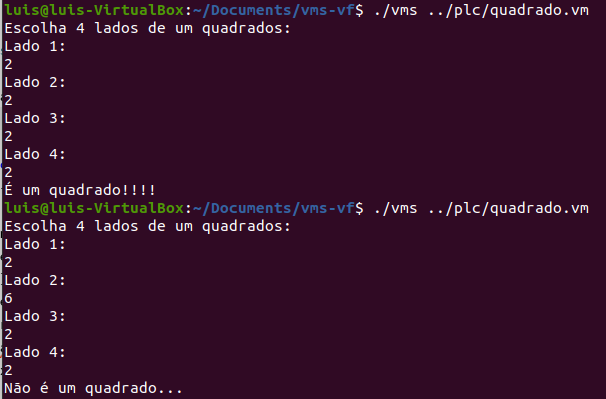
\includegraphics[width=10cm,height=6cm]{Quadrado.jpeg}
\caption{Quadrado.jpeg}
\end{figure}

%%%%%%%%%%%%%%%%%%%%%%%%%%%%%%%%%%%%%%% 4.2

\subsection{Menor} %subseccao
\setlength{\parindent}{5ex} 
\par Este programa lê um inteiro N, depois lê N números e escreve o menor deles

\begin{lstlisting}[firstnumber=0]
Int -> n,i,m:50000000;

Main ->
	
	n:read("Escolha um número inteiro positivo:");

	?(n<=0)->
		write("Valor inválido!");
	;->>
		W?(n>0)->
			write("Escreva um número:");
			i:read();
			?(i<m)->
				m:i;
			;
			n:n-1;
		;
		write("Menor número:",m);
	;
;
\end{lstlisting}

Código Assembly da VM gerado:

\begin{lstlisting}[firstnumber=0]
PUSHI 0
PUSHI 0
PUSHI 50000000
START
PUSHS "Escolha um número inteiro positivo:"
WRITES
PUSHS "\n"
WRITES
READ
ATOI
STOREG 0
E4: nop
PUSHG 0
PUSHI 0
INFEQ
JZ E5
PUSHS "Valor inválido!"
WRITES
PUSHS "\n"
WRITES
JUMP E6
E5: nop
E2: nop
PUSHG 0
PUSHI 0
SUP
JZ E3
PUSHS "Escreva um número:"
WRITES
PUSHS "\n"
WRITES
READ
ATOI
STOREG 1
E0: nop
PUSHG 1
PUSHG 2
INF
JZ E1
PUSHG 1
STOREG 2
E1: nop
PUSHG 0
PUSHI 1
SUB
STOREG 0
JUMP E2
E3: nop
PUSHS "Menor número:"
WRITES
PUSHS "\n"
WRITES
PUSHG 2
WRITEI
PUSHS "\n"
WRITES
E6: nop
STOP
\end{lstlisting}

Programa a ser executado pela VM:
\begin{figure}[h]
\centering
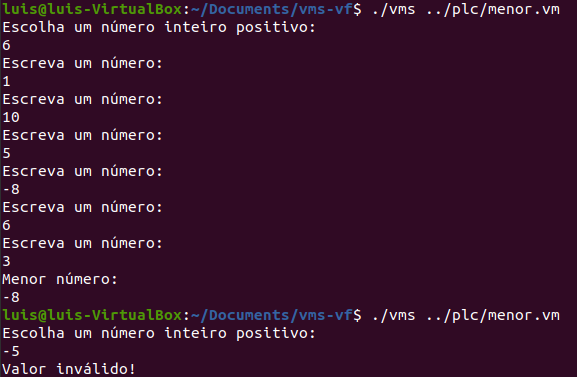
\includegraphics[width=8cm,height=6cm]{Menor.jpeg}
\caption{Menor.jpeg}
\end{figure}

%%%%%%%%%%%%%%%%%%%%%%%%%%%%%%%%%%%%%%%%%%%%%%

\subsection{Produtório} %subseccao
\setlength{\parindent}{5ex}
\par Este programa lê um inteiro N, depois lê N números e calcula o seu produtório

\begin{lstlisting}[firstnumber=0]
Int -> n,p:1,i;

Main ->
	n:read("Quantos números quer multiplicar?");

	?(n<=0)->
		write("Valor inválido!");
	;->>
		W?(n>0)->
			write("Escreva um número:");
			i:read();
			p:p*i;
			n:n-1;
		;
		write("Produtório:",p);
	;
;
\end{lstlisting}

Código Assembly da VM gerado:
\begin{lstlisting}[firstnumber=0]
PUSHI 0
PUSHI 1
PUSHI 0
START
PUSHS "Quantos números quer multiplicar?"
WRITES
PUSHS "\n"
WRITES
READ
ATOI
STOREG 0
E2: nop
PUSHG 0
PUSHI 0
INFEQ
JZ E3
PUSHS "Valor inválido!"
WRITES
PUSHS "\n"
WRITES
JUMP E4
E3: nop
E0: nop
PUSHG 0
PUSHI 0
SUP
JZ E1
PUSHS "Escreva um número:"
WRITES
PUSHS "\n"
WRITES
READ
ATOI
STOREG 2
PUSHG 1
PUSHG 2
MUL
STOREG 1
PUSHG 0
PUSHI 1
SUB
STOREG 0
JUMP E0
E1: nop
PUSHS "Produtório:"
WRITES
PUSHS "\n"
WRITES
PUSHG 1
WRITEI
PUSHS "\n"
WRITES
E4: nop
STOP
\end{lstlisting}

Programa a ser executado pela VM:
\begin{figure}[h]
\centering
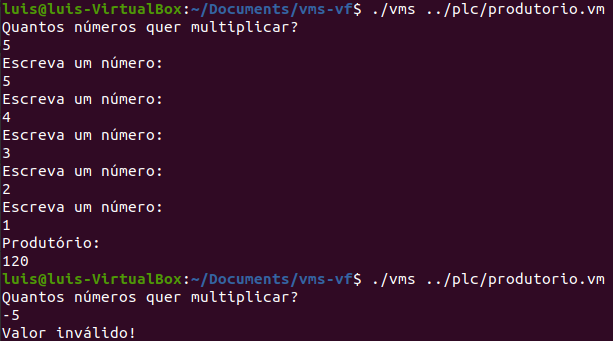
\includegraphics[width=10cm,height=6cm]{Produtorio.jpeg}
\caption{Produtorio.jpeg}
\end{figure}

%%%%%%%%%%%%%%%%%%%%%%%%%%%%%%%%%%%%%%%%%%%%%%% 4.4

\subsubsection{Sequência}
\setlength{\parindent}{5ex}
Este programa conta e imprime os números ímpares de uma sequência de números naturais.

\begin{lstlisting}
Int -> n,conta:0,i;

Main ->

	n:read("Qual é o tamanho da sua sequência?");
	
	?(n<=0)->
		write("Valor inválido!");
	;->>

		W?(n>0)->

			i:read("Escreva um número natural:");

			?(i<0)->
				write("Tem de ser um número natural!");
			
			;->>

				?(i % 2 = 1)->
					conta : conta + 1;
					write("Encontrado um número ímpar:",i);
				;
				n:n-1;	
			;
			
		;

		write("Foi encontrado um total de números ímpares igual a:",conta);
	;
;
\end{lstlisting}

Código Assembly da VM gerado:
\begin{lstlisting}[firstnumber=1]
PUSHI 0
PUSHI 0
PUSHI 0
START
PUSHS "Qual é o tamanho da sua sequência?"
WRITES
PUSHS "\n"
WRITES
READ
ATOI
STOREG 0
E7: nop
PUSHG 0
PUSHI 0
INFEQ
JZ E8
PUSHS "Valor inválido!"
WRITES
PUSHS "\n"
WRITES
JUMP E9
E8: nop
E5: nop
PUSHG 0
PUSHI 0
SUP
JZ E6
PUSHS "Escreva um número natural:"
WRITES
PUSHS "\n"
WRITES
READ
ATOI
STOREG 2
E2: nop
PUSHG 2
PUSHI 0
INF
JZ E3
PUSHS "Tem de ser um número natural!"
WRITES
PUSHS "\n"
WRITES
JUMP E4
E3: nop
E0: nop
PUSHG 2
PUSHI 2
MOD
PUSHI 1
EQUAL
JZ E1
PUSHG 1
PUSHI 1
ADD
STOREG 1
PUSHS "Encontrado um número ímpar:"
WRITES
PUSHS "\n"
WRITES
PUSHG 2
WRITEI
PUSHS "\n"
WRITES
E1: nop
PUSHG 0
PUSHI 1
SUB
STOREG 0
E4: nop
JUMP E5
E6: nop
PUSHS "Foi encontrado um total de números ímpares igual a:"
WRITES
PUSHS "\n"
WRITES
PUSHG 1
WRITEI
PUSHS "\n"
WRITES
E9: nop
STOP
\end{lstlisting}

\clearpage
Programa a ser executado pela VM:
\begin{figure}[h]
\centering
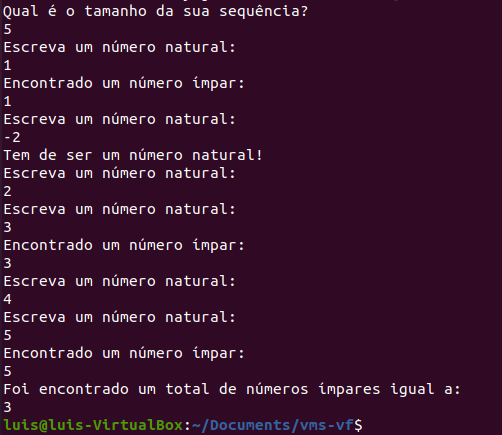
\includegraphics[width=10cm,height=10cm]{Sequencia.jpeg}
\caption{Sequencia.jpeg}
\end{figure}


\subsection{Inverter} %subseccao
\setlength{\parindent}{5ex}

\par Este programa lê e armazena N números num array e depois imprime-o por ordem inversa.

\begin{lstlisting}
Int -> i,aux;

Array -> a:6;

Main ->
	write("Escreva os 6 elementos do array:");
	
	W?(i<6)->
		a[i]:read();
		i:i+1;
	;

	write("Array Invertido:");

	i:i-1;

	W?(i>=0)->
		aux:a[i];
		write(aux);
		i:i-1;
	;
;
\end{lstlisting}


\par Código Assembly da VM gerado:
\begin{lstlisting}
PUSHI 0
PUSHI 0
PUSHN 6
START
PUSHS "Escreva os 6 elementos do array:"
WRITES
PUSHS "\n"
WRITES
E0: nop
PUSHG 0
PUSHI 6
INF
JZ E1
PUSHGP
PUSHI 2
PADD
PUSHG 0
CHECK 0 6
READ
ATOI
STOREN
PUSHG 0
PUSHI 1
ADD
STOREG 0
JUMP E0
E1: nop
PUSHS "Array Invertido:"
WRITES
PUSHS "\n"
WRITES
PUSHG 0
PUSHI 1
SUB
STOREG 0
E2: nop
PUSHG 0
PUSHI 0
SUPEQ
JZ E3
PUSHGP
PUSHI 2
PADD
PUSHG 0
CHECK 0 5
LOADN
STOREG 1
PUSHG 1
WRITEI
PUSHS "\n"
WRITES
PUSHG 0
PUSHI 1
SUB
STOREG 0
JUMP E2
E3: nop
STOP
\end{lstlisting}

Programa a ser executado pela VM:
\begin{figure}[h]
\centering
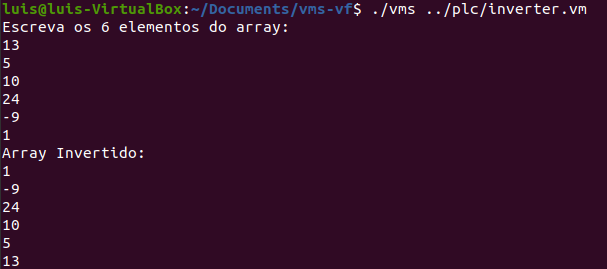
\includegraphics[width=10cm,height=5cm]{Inverter.jpeg}
\caption{Inverter.jpeg}
\end{figure}

\clearpage


%%%%%%%%%%%%%%%%%%%%%%%%%%%%%%%%%%%%%%%%%%%%%%%%%%%%%%%%%%

\vspace{1CM}

\section{Conclusão} \label{sec:Conclusão}
\setlength{\parindent}{5ex} Através deste trabalho prático foi-nos possível pôr em prática o conhecimento sobre \tt{LeX}, \tt{Yacc} e o módulo {\tt ply} de Python dados durante as aulas, bem como a sua aplicação real na criação de uma linguagem de programação e o respectivo compilador.
\par Fazemos uma avaliação positiva do nosso desempenho neste projeto pois achamos que o objetivo do mesmo foi concluído. Apesar de alguns desafios encontrados na sua realização, estes foram superados com distinção, revelando assim um trabalho consistente e bem estruturado.

\clearpage

\appendix
\section{Código do Programa}
\subsection{Lex}

\begin{lstlisting}[language=Python]
import ply.lex as lex
import sys


tokens = ('MAIN',    
          'SETA',    
          'LPAREN',  
          'RPAREN',  
          'WHILE',   
          'IF',      
          'ELSE',    
          'DP',      
          'INT',     
          'ARR',     
          'NUMI',    
          'ID',      
          'VIR',     
          'AND',     
          'OR',      
          'NOT',     
          'EQ',      
          'NEQ',     
          'LE',      
          'GE',      
          'MENOR',   
          'MAIOR',   
          'MAIS',    
          'MENOS',   
          'MUL',     
          'DIV',     
          'RESDI',   
          'PV',      
          'READ',    
          'WRITE',   
          'STRING',  
          'NL',      
          'LPARENR', 
          'RPARENR'  
        )

t_EQ = r'\='
t_MAIOR = r'\>'
t_MENOR = r'\<'
t_MENOS = r'\-'
t_MAIS = r'\+'
t_MUL = r'\*'
t_DIV = r'\/'
t_RESDI = r'\%'
t_PV = r';'
t_VIR = r','
t_DP = r':'
t_IF = r'\?'
t_LPAREN = r'\('
t_RPAREN = r'\)'
t_LPARENR = r'\['
t_RPARENR = r'\]'
t_SETA = r'\->'
t_ID = r'[a-z][a-zA-Z]*'


def t_NEQ(t):
    r'\!\='
    return t

def t_ELSE(t):
    r'\->>'
    return t

def t_MAIN(t): 
    r'Main'
    return t

def t_WHILE(t):
    r'W\?'
    return t

def t_INT(t):
    r'Int'
    return t

def t_ARR(t):
    r'Array'
    return t

def t_WRITE(t):
    r'write'
    return t

def t_READ(t):
    r'read'
    return t

def t_STRING(t):
    r'\"[^\"]*\"'
    return t

def t_NUMI(t):
    r'[0-9]+'
    t.value = int(t.value)
    return t

def t_AND(t):
    r'and'
    return t

def t_OR(t):
    r'or'
    return t

def t_NOT(t):
    r'\!'
    return t

def t_LE(t):
    r'\<\='
    return t

def t_GE(t):
    r'\>\='
    return t

def t_NL(t):
    r'\n'
    t.lexer.lineno += len(t.value)
    return t

t_ignore = ' \t'

def t_error(t):
    print("Illegal character {} at line {}".format(t.value[0], t.lineno,))
    t.lexer.skip(1)

lexer = lex.lex()
\end{lstlisting}

\subsection{Yacc}

\begin{lstlisting}[language=Python]
import ply.yacc as yacc
import sys

from plclex import tokens


def p_prog(p):
    "Prog : Decls Main"
    print(p[1]+p[2])


########################## GIC para as declaraçoes
def p_decls(p):
    "Decls : Decls Decl"
    p[0] = p[1] + p[2]

def p_decls_empty(p):
    "Decls : "
    p[0] = ''


def p_decl_int(p):
    "Decl : INT SETA DeclList PV NL"
    p[0] = p[3]

def p_decl_array(p):
    "Decl : ARR SETA ArrayList PV NL"
    p[0] = p[3]

def p_decl_nl(p):
    "Decl : NL"
    p[0] = ''


def p_decllist(p):
    "DeclList : UniDecl VIR DeclList"
    p[0] = p[1] + p[3]

def p_decllist_uni(p):
    "DeclList : UniDecl"
    p[0] = p[1]

def p_arraylist(p):
    "ArrayList : Array VIR ArrayList"
    p[0] = p[1] + p[3]

def p_arraylist_uni(p):
    "ArrayList : Array"
    p[0] = p[1]


def p_unidecl_id(p): 
    "UniDecl : ID"
    if p[1] in parser.tabID:
        string = "Erro semântico: Var " + p[1] + " já está definida!"
        p[0] = r'ERR "' + string + '"' + '\n' + 'STOP' + '\n'
    
    else:
        parser.tabID.update({p[1] : (parser.proxE,0,"Int")})
        parser.proxE += 1
        p[0] = r'PUSHI 0' + '\n'


def p_unidecl_atr(p):
    "UniDecl : ID DP NUMI"
    if p[1] in parser.tabID:
        string = "Erro semântico: Var " + p[1] + " já está definida!"
        p[0] = r'ERR "' + string + '"' + '\n' + 'STOP' + '\n'
    
    else:
        parser.tabID.update({p[1] : (parser.proxE,p[3],"Int")})
        parser.proxE += 1
        p[0] = r'PUSHI '+ str(p[3]) + '\n'


def p_unidecl_atrn(p):
    "UniDecl : ID DP MENOS NUMI"
    if p[1] in parser.tabID:
        string = "Erro semântico: Var " + p[1] + " já está definida!"
        p[0] = r'ERR "' + string + '"' + '\n' + 'STOP' + '\n'
    
    else:
        parser.tabID.update({p[1] : (parser.proxE,-p[4],"Int")})
        parser.proxE += 1
        p[0] = r'PUSHI '+ str(-p[4]) + '\n'


def p_arrayAtr(p):
    "Array : ID DP NUMI"
    if p[1] in parser.tabID:
        string = "Erro semântico: Var " + p[1] + " já está definida!"
        p[0] = r'ERR "' + string + '"' + '\n' + 'STOP' + '\n'
    
    else:
        parser.tabID.update({p[1] : (parser.proxE,p[3],"Array")})    #(end do inicio do array,tamanho,tipo da var Array)
        parser.proxE += p[3]
        p[0] = r'PUSHN ' + str(p[3]) + '\n'


def p_arrayAtrlist(p):
    "Array : ID DP List"
    if p[1] in parser.tabID:
        string = "Erro semântico: Var " + p[1] + " já está definida!"
        p[0] = r'ERR "' + string + '"' + '\n' + 'STOP' + '\n'
    
    else:
        p[0] = p[3]
        parser.tabID.update({p[1] : (parser.proxE-parser.conta,parser.conta,"Array")})
        parser.conta = 0

def p_arrayAtrlist2(p):
    "List : LPARENR Nums RPARENR"
    p[0] = p[2]

def p_elems(p):
    "Nums : Nums VIR Num"
    parser.conta += 1
    p[0] = p[1] + p[3]

def p_elems2(p):
    "Nums : Num"
    parser.conta = 1
    p[0] = p[1]

def p_elems3(p):
    "Num : NUMI"
    p[0] = r'PUSHI ' + str(p[1]) + '\n'
    parser.proxE += 1

def p_elems4(p):
    "Num : MENOS NUMI"
    p[0] = r'PUSHI ' + str(-p[2]) + '\n'
    parser.proxE += 1


########################## GIC para a main function
def p_main(p):
    "Main : MAIN SETA NL Instrs PV"
    p[0] = r'START' + '\n' + p[4] + r'STOP'


########################## GIC para instructions
def p_instrs(p):
    "Instrs : Instrs Instr"
    p[0] = p[1] + p[2]

def p_instrs_empty(p):
    "Instrs : "
    p[0] = ''


def p_instr_atr(p):
    "Instr : Atr NL"
    p[0] = p[1]

def p_instr_cond(p):
    "Instr : Cond NL"
    p[0] = p[1]

def p_instr_ciclo(p):
    "Instr : Ciclo NL"
    p[0] = p[1]

def p_instr_write(p):
    "Instr : Write NL"
    p[0] = p[1]

def p_instr_nl(p):
    "Instr : NL"
    p[0] = ''


########################## GIC para atribuiçoes
def p_atrib(p):
    "Atr : ID DP Expr PV"
    if p[1] not in parser.tabID:
        string = "Erro semântico: Var " + str(p[1]) + " não está definida!"
        p[0] = r'ERR "' + string + '"' + '\n' + 'STOP' + '\n'

    elif parser.tabID[p[1]][2]!="Int":
        string = "Erro semântico: Var " + str(p[1]) + " não é do tipo inteiro!"
        p[0] = r'ERR "' + string + '"' + '\n' + 'STOP' + '\n'     
    
    else:
        p[0] = p[3] + r'STOREG ' + str(parser.tabID[p[1]][0]) + '\n'
    

def p_atrib_read(p):
    "Atr : ID DP Read"
    if p[1] not in parser.tabID:
        string = "Erro semântico: Var " + str(p[1]) + " não está definida!"
        p[0] = r'ERR "' + string + '"' + '\n' + 'STOP' + '\n'

    elif parser.tabID[p[1]][2]!="Int":
        string = "Erro semântico: Var " + str(p[1]) + " não é do tipo inteiro!"
        p[0] = r'ERR "' + string + '"' + '\n' + 'STOP' + '\n'

    else:
        p[0] = p[3] + r'STOREG ' + str(parser.tabID[p[1]][0]) + '\n'


def p_atribarray_numi(p):
    "Atr : ID LPARENR NUMI RPARENR DP Expr PV"
    if p[1] not in parser.tabID:
        string = "Erro semântico: Var " + str(p[1]) + " não está definida!"
        p[0] = r'ERR "' + string + '"' + '\n' + 'STOP' + '\n'

    elif parser.tabID[p[1]][2]!="Array":
        string = "Erro semântico: Var " + str(p[1]) + " não é do tipo array!"
        p[0] = r'ERR "' + string + '"' + '\n' + 'STOP' + '\n'

    elif p[3]>=parser.tabID[p[1]][1]:
        string = "Erro semântico: " + p[3] + " encontra-se fora do limite do tamanho do array!"
        p[0] = r'ERR "' + string + '"' + '\n' + 'STOP' + '\n'

    else:
        p[0] = p[6] + r'STOREG ' + str(parser.tabID[p[1]][0]+p[3]) + '\n'


def p_atribarray_numi_read(p):
    "Atr : ID LPARENR NUMI RPARENR DP Read"
    if p[1] not in parser.tabID:
        string = "Erro semântico: Var " + str(p[1]) + " não está definida!"
        p[0] = r'ERR "' + string + '"' + '\n' + 'STOP' + '\n'

    elif parser.tabID[p[1]][2]!="Array":
        string = "Erro semântico: Var " + str(p[1]) + " não é do tipo array!"
        p[0] = r'ERR "' + string + '"' + '\n' + 'STOP' + '\n'

    else:
        p[0] = p[6] + r'STOREG ' + str(parser.tabID[p[1]][0]+p[3]) + '\n'


def p_atribarray_id(p):
    "Atr : ID LPARENR ID RPARENR DP Expr PV"
    if p[1] not in parser.tabID:
        string = "Erro semântico: Var " + str(p[1]) + " não está definida!"
        p[0] = r'ERR "' + string + '"' + '\n' + 'STOP' + '\n'

    elif parser.tabID[p[1]][2]!="Array":
        string = "Erro semântico: Var " + str(p[1]) + " não é do tipo array!"
        p[0] = r'ERR "' + string + '"' + '\n' + 'STOP' + '\n'

    elif p[3] not in parser.tabID:
        string = "Erro semântico: Var " + str(p[3]) + " não está definida!"
        p[0] = r'ERR "' + string + '"' + '\n' + 'STOP' + '\n'

    elif parser.tabID[p[3]][2]!="Int":
        string = "Erro semântico: Var " + str(p[1]) + " não é do tipo inteiro!"
        p[0] = r'ERR "' + string + '"' + '\n' + 'STOP' + '\n'

    else:
        p[0] = r'PUSHGP' + '\n' + \
               r'PUSHI ' + str(parser.tabID[p[1]][0]) + '\n' + \
               r'PADD' + '\n' + \
               r'PUSHG ' + str(parser.tabID[p[3]][0]) + '\n' + \
               r'CHECK ' + '0 ' + str(parser.tabID[p[1]][1]-1) + '\n' + \
               p[6] + \
               r'STOREN' + '\n'


def p_atribarray_read(p):
    "Atr : ID LPARENR ID RPARENR DP Read"
    if p[1] not in parser.tabID:
        string = "Erro semântico: Var " + str(p[1]) + " não está definida!"
        p[0] = r'ERR "' + string + '"' + '\n' + 'STOP' + '\n'

    elif parser.tabID[p[1]][2]!="Array":
        string = "Erro semântico: Var " + str(p[1]) + " não é do tipo array!"
        p[0] = r'ERR "' + string + '"' + '\n' + 'STOP' + '\n'

    elif p[3] not in parser.tabID:
        string = "Erro semântico: Var " + str(p[3]) + " não está definida!"
        p[0] = r'ERR "' + string + '"' + '\n' + 'STOP' + '\n'

    elif parser.tabID[p[3]][2]!="Int":
        string = "Erro semântico: Var " + str(p[1]) + " não é do tipo inteiro!"
        p[0] = r'ERR "' + string + '"' + '\n' + 'STOP' + '\n'

    else:
        p[0] = r'PUSHGP' + '\n' + \
               r'PUSHI ' + str(parser.tabID[p[1]][0]) + '\n' + \
               r'PADD' + '\n' + \
               r'PUSHG ' + str(parser.tabID[p[3]][0]) + '\n' + \
               r'CHECK ' + '0 ' + str(parser.tabID[p[1]][1]) + '\n' + \
               p[6] + \
               r'STOREN' + '\n'


########################## GIC para a function read
def p_read(p):
    "Read : READ LPAREN RPAREN PV"
    p[0] = r'READ' + '\n' + r'ATOI' + '\n'

def p_read_String(p):
    "Read : READ LPAREN String RPAREN PV"
    p[0] = r'PUSHS ' + p[3] + '\n' + r'WRITES' + '\n' + \
           r'PUSHS ' + r'"\n"' + '\n' + r'WRITES' + '\n' + \
           r'READ' + '\n' + r'ATOI' + '\n'


########################## GIC para condiçoes
def p_cond_if(p):
    "Cond : IF LPAREN Expr RPAREN SETA NL Instrs PV"
    p[0] = r'E' + str(parser.nivelC) + r': nop' + '\n' + p[3] + \
           r'JZ E' + str(parser.nivelC + 1) + '\n' + p[7] + \
           r'E' + str(parser.nivelC + 1) + r': nop' + '\n'
    parser.nivelC += 2


def p_cond_ifelse(p):
    "Cond : IF LPAREN Expr RPAREN SETA NL Instrs PV ELSE NL Instrs PV"
    p[0] = r'E' + str(parser.nivelC) + r': nop' + '\n' + p[3] + \
           r'JZ E' + str(parser.nivelC + 1) + '\n' + p[7] + 'JUMP E' + str(parser.nivelC + 2) + '\n' + \
           r'E' + str(parser.nivelC + 1) + r': nop' + '\n' + p[11] + \
           r'E' + str(parser.nivelC + 2) + r': nop' + '\n'
    parser.nivelC += 3


########################## GIC para ciclos
def p_ciclo(p):
    "Ciclo : WHILE LPAREN Expr RPAREN SETA NL Instrs PV"
    p[0] = r'E' + str(parser.nivelC) + r': nop' + '\n' + p[3] + \
           r'JZ E' + str(parser.nivelC + 1) + '\n' + p[7] + 'JUMP E' + str(parser.nivelC) + '\n' + \
           r'E' + str(parser.nivelC + 1) + r': nop' + '\n'
    parser.nivelC += 2


########################## GIC para a function write
def p_write_string(p):
    "Write : WRITE LPAREN String RPAREN PV"   
    p[0] = r'PUSHS ' + p[3] + '\n' + r'WRITES' + '\n' + r'PUSHS ' + r'"\n"' + '\n' + r'WRITES' + '\n'

def p_write_args(p):
    "Write : WRITE LPAREN String VIR ListArgs RPAREN PV"
    p[0] = r'PUSHS ' + p[3] + '\n' + r'WRITES' + '\n' + r'PUSHS ' + r'"\n"' + '\n' + r'WRITES' + '\n' + p[5]

def p_write_id(p):
    "Write : WRITE LPAREN ID RPAREN PV"
    if p[3] not in parser.tabID:
        string = "Erro semântico: Var " + p[3] + " não está definida!" + '\n'
        p[0] = r'ERR "' + string + '"' + '\n' + 'STOP' + '\n'

    elif parser.tabID[p[3]][2]=="Int":
        p[0] = r'PUSHG ' + str(parser.tabID[p[3]][0]) + '\n' + r'WRITEI' + '\n' + r'PUSHS ' + r'"\n"' + '\n' + r'WRITES' + '\n'

    elif parser.tabID[p[3]][2]=="Array":
        aux = 0
        s = ''
        while aux<parser.tabID[p[3]][1]:
            s += r'PUSHG ' + str(parser.tabID[p[3]][0]+aux) + '\n' + r'WRITEI' + '\n' + r'PUSHS ' + r'"\n"' + '\n' + r'WRITES' + '\n'
            aux += 1
        p[0] = s


def p_string(p):
    "String : STRING"
    p[0] = str(p[1])

def p_listargs(p):
    "ListArgs : ListArgs VIR Elem"
    p[0] = p[1] + p[3]

def p_listargs_uno(p):
    "ListArgs : Elem"
    p[0] = p[1]


def p_elem_id(p):
    "Elem : ID"
    if p[1] not in parser.tabID:
        string = "Erro semântico: Var " + str(p[1]) + " não está definida!"
        p[0] = r'ERR "' + string + '"' + '\n' + 'STOP' + '\n'

    elif parser.tabID[p[1]][2]!="Int":
        string = "Erro semântico: Var " + str(p[1]) + " não é do tipo inteiro!"
        p[0] = r'ERR "' + string + '"' + '\n' + 'STOP' + '\n'

    else:
        p[0] = r'PUSHG ' + str(parser.tabID[p[1]][0]) + '\n' + r'WRITEI' + '\n' + r'PUSHS ' + r'"\n"' + '\n' + r'WRITES' + '\n'


########################## GIC para Expressoes
def p_expr_and(p):
    "Expr : Expr AND LExpr"
    p[0] = p[1] + p[3] + r'MUL' + '\n' + \
           r'PUSHI 0' + '\n' + r'EQUAL' + '\n' + r'NOT' + '\n'

def p_expr_or(p):
    "Expr : Expr OR LExpr"
    p[0] = p[1] + p[3] + r'ADD' + '\n' + \
           r'PUSHI 0' + '\n' + r'EQUAL' + '\n' + r'NOT' + '\n' 

def p_expr_not(p):
    "Expr : NOT LExpr"
    p[0] = p[2] + r'NOT' + '\n'

def p_expr(p):
    "Expr : LExpr"
    p[0] = p[1]


########################## GIC para Expressoes Logicas
def p_lexpr_eq(p):
    "LExpr : LExpr EQ AritE"
    p[0] = p[1] + p[3] + r'EQUAL' + '\n'

def p_lexpr_neq(p):
    "LExpr : LExpr NEQ AritE"
    p[0] = p[1] + p[3] + r'EQUAL' + '\n' + r'NOT'+ '\n'

def p_lexpr_ge(p):
    "LExpr : LExpr GE AritE"
    p[0] = p[1] + p[3] + r'SUPEQ' + '\n'

def p_lexpr_LE(p):
    "LExpr : LExpr LE AritE"
    p[0] = p[1] + p[3] + r'INFEQ' + '\n'

def p_lexpr_maior(p):
    "LExpr : LExpr MAIOR AritE"
    p[0] = p[1] + p[3] + r'SUP' + '\n'

def p_lexpr_menor(p):
    "LExpr : LExpr MENOR AritE"
    p[0] = p[1] + p[3] + r'INF' + '\n'

def p_lexpr(p):
    "LExpr : AritE"
    p[0] = p[1]


########################## GIC para Espressoes Aritmeticas
def p_arite_mais(p):
    "AritE : AritE MAIS Termo"
    p[0] = p[1] + p[3] + r'ADD' + '\n'

def p_arite_menos(p):
    "AritE : AritE MENOS Termo"
    p[0] = p[1] + p[3] + r'SUB' + '\n'

def p_arite(p):
    "AritE : Termo"
    p[0] = p[1]


def p_termo_mul(p):
    "Termo : Termo MUL Parc"
    p[0] = p[1] + p[3] + r'MUL' + '\n'

def p_termo_div(p):
    "Termo : Termo DIV Parc"
    p[0] = p[1] + p[3] + r'DIV' + '\n'

def p_termo_divi(p):
    "Termo : Termo RESDI Parc"
    p[0] = p[1] + p[3] + r'MOD' + '\n'

def p_termo(p):
    "Termo : Parc"
    p[0] = p[1]


def p_parc_exp(p):
    "Parc : LPAREN Expr RPAREN"
    p[0] = p[2]

def p_parc(p):
    "Parc : Fator"
    p[0] = p[1]


def p_fator_numi(p):
    "Fator : NUMI"
    p[0] = r'PUSHI ' + str(p[1]) + '\n'

def p_fator_numin(p):
    "Fator : MENOS NUMI"
    p[0] = r'PUSHI ' + str(-p[2]) + '\n'


def p_fator_id(p):
    "Fator : ID"
    if p[1] not in parser.tabID:
        string = "Erro semântico: Var " + str(p[1]) + " não está definida!"
        p[0] = r'Err "' + string + '"' + '\n' + 'STOP'  + '\n'

    elif parser.tabID[p[1]][2]!="Int":
        string = "Erro semântico: Var " + str(p[1]) + " não é do tipo inteiro!"
        p[0] = r'Err "' + string + '"' + '\n' + 'STOP'  + '\n'

    else:
        p[0] = r'PUSHG ' + str(parser.tabID[p[1]][0]) + '\n'

def p_fator_idn(p):
    "Fator : MENOS ID"
    if p[2] not in parser.tabID:
        string = "Erro semântico: Var " + str(p[2]) + " não está definida!"
        p[0] = r'Err "' + string + '"' + '\n' + 'STOP'  + '\n'

    elif parser.tabID[p[2]][2]!="Int":
        string = "Erro semântico: Var " + str(p[2]) + " não é do tipo inteiro!"
        p[0] = r'Err "' + string + '"' + '\n' + 'STOP'  + '\n'
    
    else:
        p[0] = r'PUSHG ' + str(parser.tabID[p[2]][0]) + '\n' + r'PUSHI -1' + '\n' + r'MUL' + '\n'
    

def p_fator_array(p):
    "Fator : ID LPARENR NUMI RPARENR" 
    if p[1] not in parser.tabID:
        string = "Erro semântico: Var " + str(p[1]) + " não está definida!"
        p[0] = r'Err "' + string + '"' + '\n' + 'STOP'  + '\n'

    elif parser.tabID[p[1]][2]!="Array":
        string = "Erro semântico: Var " + str(p[1]) + " não é do tipo array!"
        p[0] = r'Err "' + string + '"' + '\n' + 'STOP'  + '\n'

    else:
        p[0] = r'PUSHGP' + '\n' + \
               r'PUSHI ' + str(parser.tabID[p[1]][0]) + '\n' + \
               r'PADD' + '\n' + \
               r'PUSHI ' + str(p[3]) + '\n' + \
               r'CHECK ' + '0 ' + str(parser.tabID[p[1]][1]-1) + '\n' \
               r'LOADN' + '\n'
        

def p_fator_array2(p):
    "Fator : ID LPARENR ID RPARENR"
    if p[1] not in parser.tabID:
        string = "Erro semântico: Var " + str(p[1]) + " não está definida!"
        p[0] = r'Err "' + string + '"' + '\n' + 'STOP'  + '\n'

    elif parser.tabID[p[1]][2]!="Array":
        string = "Erro semântico: Var " + str(p[1]) + " não é do tipo array!"
        p[0] = r'Err "' + string + '"' + '\n' + 'STOP'  + '\n'

    elif p[3] not in parser.tabID:
        string = "Erro semântico: Var " + str(p[3]) + " não está definida!"
        p[0] = r'Err "' + string + '"' + '\n' + 'STOP'  + '\n'

    elif parser.tabID[p[3]][2]!="Int":
        string = "Erro semântico: Var " + str(p[3]) + " não é do tipo inteiro!"
        p[0] = r'Err "' + string + '"' + '\n' + 'STOP'  + '\n'

    else:
        p[0] = r'PUSHGP' + '\n' + \
               r'PUSHI ' + str(parser.tabID[p[1]][0]) + '\n' + \
               r'PADD' + '\n' + \
               r'PUSHG ' + str(parser.tabID[p[3]][0]) + '\n' + \
               r'CHECK ' + '0 ' + str(parser.tabID[p[1]][1]-1) + '\n' \
               r'LOADN' + '\n'


########################## ERRO
def p_error(p):
    print("Syntax error: ", p)
    parser.exito = False

parser = yacc.yacc()
parser.tabID = {}   
parser.proxE = 0
parser.nivelC = 0
parser.conta = 0

parser.exito = True

fonte = ""

name = input()
name += '.txt'

with open(name,'r') as f:
    for line in f:
        fonte+=line

'''
for linha in sys.stdin:
    fonte += linha
'''

parser.parse(fonte)

#if parser.exito:
#    print ("Parsing teminou com sucesso!")
\end{lstlisting}

\clearpage
\section{Gramática}

\begin{lstlisting}
Prog :  Decls Main

Decls : Delcs Decl
      | € 

Decl : INT SETA DeclList PV NL
     | ARR SETA ArrayList PV NL
     | NL

DeclList : UniDecl VIR DecList
         | UniDecl

ArrayList : Array VIR ArrayList
          | Array

UniDecl : ID
        | ID DP NUMI
        | ID DP MENOS NUMI

Array : ID DP NUMI
	  | ID DP List

List : LPARENR Nums RPARENR

Nums : Nums VIR Num
     | Num

Num : NUMI
    | MENOS NUMI 

Main : MAIN SETA NL Instrs PV

Instrs : Instrs Instr
       | €

Instr : Atr NL
      | Cond NL
      | Ciclo NL
      | Write NL
      | NL

Atr : ID DP Expr PV
    | ID DP Read
    | ID LPARENR NUMI RPARENR DP Expr PV
    | ID LPARENR NUMI RPARENR DP Read
    | ID LPARENR ID RPARENR DP Expr PV
    | ID LPARENR ID RPARENR DP Read

Read : READ LPAREN RPAREN PV
     | READ LPAREN String RPAREN PV

Cond : IF LPAREN Expr RPAREN SETA NL Instrs PV
     | IF LPAREN Expr RPAREN SETA NL Instrs PV ELSE NL Instrs PV

Ciclo : WHILE LPAREN Expr RPAREN SETA NL Instrs PV

Write : WRITE LPAREN String RPAREN PV
      | WRITE LPAREN String VIR ListArgs RPAREN PV
      | WRITE LPAREN ID RPAREN PV

String : STRING

ListaArgs : ListArgs VIR Elem 
          | Elem

Elem : ID

Expr : Expr AND LExpr
     | Expr OR LExpr
     | NOT LExpr
     | LExpr

LExpr : LExpr EQ AritE
      | LExpr NEQ AritE
      | LExpr GE AritE
      | LExpr LE AritE
      | LExpr MAIOR AritE
      | LExpr MENOR AritE
      | AritE

AritE : AritE MAIS Termo
      | AritE MENOS Termo
      | Termo

Termo : Termo MUL Parc
      | Termo DIV Parc
      | Termo RESDI Parc
      | Parc

Parc : LPAREN Expr RPAREN
     | Fator


Fator : NUMI
      | MENOS NUMI
      | ID
      | MENOS ID
      | ID LPARENR NUMI RPARENR
      | ID LPARENR ID RPARENR
\end{lstlisting}
\end{document}


